\section {Regression Analysis and Modeling}
\label{sec:regression}
\nocite{valdivia2011simple}

\renewcommand{\loadeq}[1]{%
   \ExecuteMetaData[./equations/regression.tex]{eq#1}%
}

Once the circuitry described in Section: \ref{sec:measCirc} collects the data for a capacitor, an analysis is needed to relate that information to the physical characteristics described in Section: \ref{sec:params}. Various models, such as in Figures: \ref{fig:fullModel} \& \ref{fig:superCap}, can be used to represent a capacitor. They differ based upon the type of capacitor, the input parameters of interest, and the desired accuracy. This section demonstrates a regression analysis technique which fits a capacitor model to the impedance data shown in Figure: \ref{fig:exCapData}. The accuracy of these fits will be evaluated to determine the model's effectiveness. See Appendix: \ref{app:genModelingImages} for the code used to generate the images shown in this section.

% This figure was generated by ./scripts/modeling/plot_ExCapData.m
\begin{figure}[ht!]
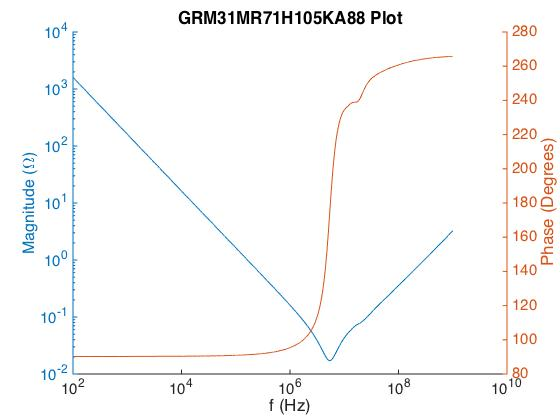
\includegraphics[keepaspectratio=true,width=6in]{./figures/modeling/exCapData.jpg}
\centering
\caption{GRM31MR71H105KA88 Capacitor Data}
\label{fig:exCapData}
\end{figure}


\subsection{Regression Analysis}
\label{sec:RegressionAnalysis}
\subsubsection{Basic LSE}
At its core, regression analysis is an optimization problem whose purpose is to fit the equation of a line to a data set. A commonly used regression analysis technique is called the \gls{lse}. It attempts to find a model which minimizes the squared error between an empirical set of data and itself.

The first step in applying an \gls{lse} is to choose the form of the equation that best represents the data. The equation of a line, Equation: \eqref{equ:ExLinEqu}, is chosen when only a simple linear fit is needed.
Then the squared error equation is generated, as in Equations: \eqref{equ:LSE_E2} \& \eqref{equ:LSE_E2b}.

\loadeq{ExLinEqu}
\loadeq{LSEE2}
\loadeq{LSEE2b}

In order to minimize the squared error over the data set, one needs to take the partial derivate of Equation: \eqref{equ:LSE_E2b} with respect to each of the unknown parameters, the coefficients, separately. While $a_0$ and $a_1$ will be constants in the final equation, they are treated as variables here until they are known. Conversely, all $x_i$ values are treated as constants. This results in Equations: \eqref{equ:LSE_PD1} \& \eqref{equ:LSE_PD2}.

\loadeq{LSEPD}

Up to this point most \gls{lse} methods analyze follow the same basic path. The rest of the steps will depend upon the complexity of the model and solution techniques. The following steps in the basic \gls{lse} use transformations and substitutions to solve for the unknown variables. In this case, Equation: \eqref{equ:avgb} is used to remove the summation terms from the equation.

\loadeq{avgb}

This results in Equations: \eqref{equ:LSE_sol} \& \eqref{equ:LSE_solb} with solutions shown in Equations: \eqref{equ:LSE_solc} \& \eqref{equ:LSE_sold}. The empirical data is then used to find the values of $a_0$ and $a_1$. At this point, the best fit line can be used to estimate new points on the plot or to compare against other data sets (Figure: \ref{fig:basicLSE}).

\begin{figure}[ht!]
\ifisPPT
\noindent\makebox[\textwidth]{\includegraphics[keepaspectratio=true,width=\paperwidth]{../figures/regression/basicLSE.jpg}}
\else
\includegraphics[keepaspectratio=true,width=6in]{./figures/regression/basicLSE.jpg}
\fi
\centering
\caption{Basic LSE}
\label{fig:basicLSE}
\end{figure}



\loadeq{LSEsol}
\loadeq{LSEsolb}
\loadeq{LSEsolc}
\loadeq{LSEsold}

\subsubsection{Levy's Technique - Complex Curve Fitting}
While the basic \gls{lse} technique is sufficient for many circumstances, it is not directly applicable in situations where one needs to fit a model to a complex line, such as a transfer function. Levy \cite{levy} shows an extension of the simple \gls{lse} example that is valid for a generic polynomial transfer function. This method is important because it not only allows for a complex-valued transfer function, but it also prevents the necessity of rederiving the system of equations for each new model. 

\loadeq{levyGs}

Using Equation: \eqref{equ:levy_Gs} as the generic model, Levy shows that you can use Equations: \eqref{equ:Levy_L}, \eqref{equ:Levy_S}, \eqref{equ:Levy_T}, \& \eqref{equ:Levy_U} to simplify the series of partial derivatives into a single matrix multiplication equation shown in \eqref{equ:Levy_Ans}, \eqref{equ:Levy_M}, \eqref{equ:Levy_N}, \& \eqref{equ:Levy_C}.

\loadeq{LevyL}
\loadeq{LevyS}
\loadeq{LevyT}
\loadeq{LevyU}
\loadeq{LevyAns}

\setcounter{MaxMatrixCols}{12} % Allows each row of M to fit on one line
\begin{equation}
\label{equ:Levy_M}
M = 
\begin{bmatrix}
\lambda _0 & 0          & -\lambda _2 &  0           & \lambda _4  & \cdots &  T_1    & S_2    & -T_3   & -S_4   &  T_5    & \cdots \\
0          & \lambda _2 & 0           & -\lambda _4  & 0           & \cdots & -S_2    & T_3    &  S_4   & -T_5   & -S_6    & \cdots \\
\lambda _2 & 0          & -\lambda _4 &  0           & \lambda _6  & \cdots &  T_3    & S_4    & -T_5   & -S_6   &  T_7    & \cdots \\
0          & \lambda _4 & 0           & -\lambda _6  & 0           & \cdots & -S_4    & T_5    &  S_6   & -T_7   & -S_8    & \cdots \\

\vdots     & \vdots     &  \vdots     & \vdots       & \vdots      &        &  \vdots & \vdots & \vdots & \vdots &  \vdots &        \\ 
T_1        & -S_2       & -T_3        &  S_4         & T_5         & \cdots &  U_2    & 0      & -U_4   &  0     &  U_6    & \cdots \\
S_2        &  T_3       & -S_4        & -T_5         & S_6         & \cdots &  0      & U_4    &  0     & -U_6   &  0      & \cdots \\
T_3        & -S_4       & -T_5        &  S_6         & T_7         & \cdots &  U_4    & 0      & -U_6   &  0     &  U_8    & \cdots \\
\vdots     & \vdots     &  \vdots     & \vdots       & \vdots      & \vdots &  \vdots & \vdots & \vdots & \vdots &  \vdots &        \\ 
\end{bmatrix}
~\cite{levy}[Eq.~21a]
\end{equation}
\loadeq{LevyNC}

Levy's technique works well for applications where there is a small dynamic frequency range and a small number of coefficients, but there are several problems with it.
The first problem is that for models with a wide bandwidth, the solution to Equation: \eqref{equ:Levy_Ans}, involves an ill-conditioned matrix. This means that the solution to the system of equations will experience precision errors.
The second problem is that this technique is heavily biased by high frequency data. As can be seen in Figure: \ref{fig:levy}, applying Levy's technique with a $3^{rd}$ order model provides a unusable fit to the empirical data.

% Run /scripts/regression/run_levy_iter.m with NumDeg = 3, DenDeg = 3, and iterations = 1.
\begin{figure}[ht!]
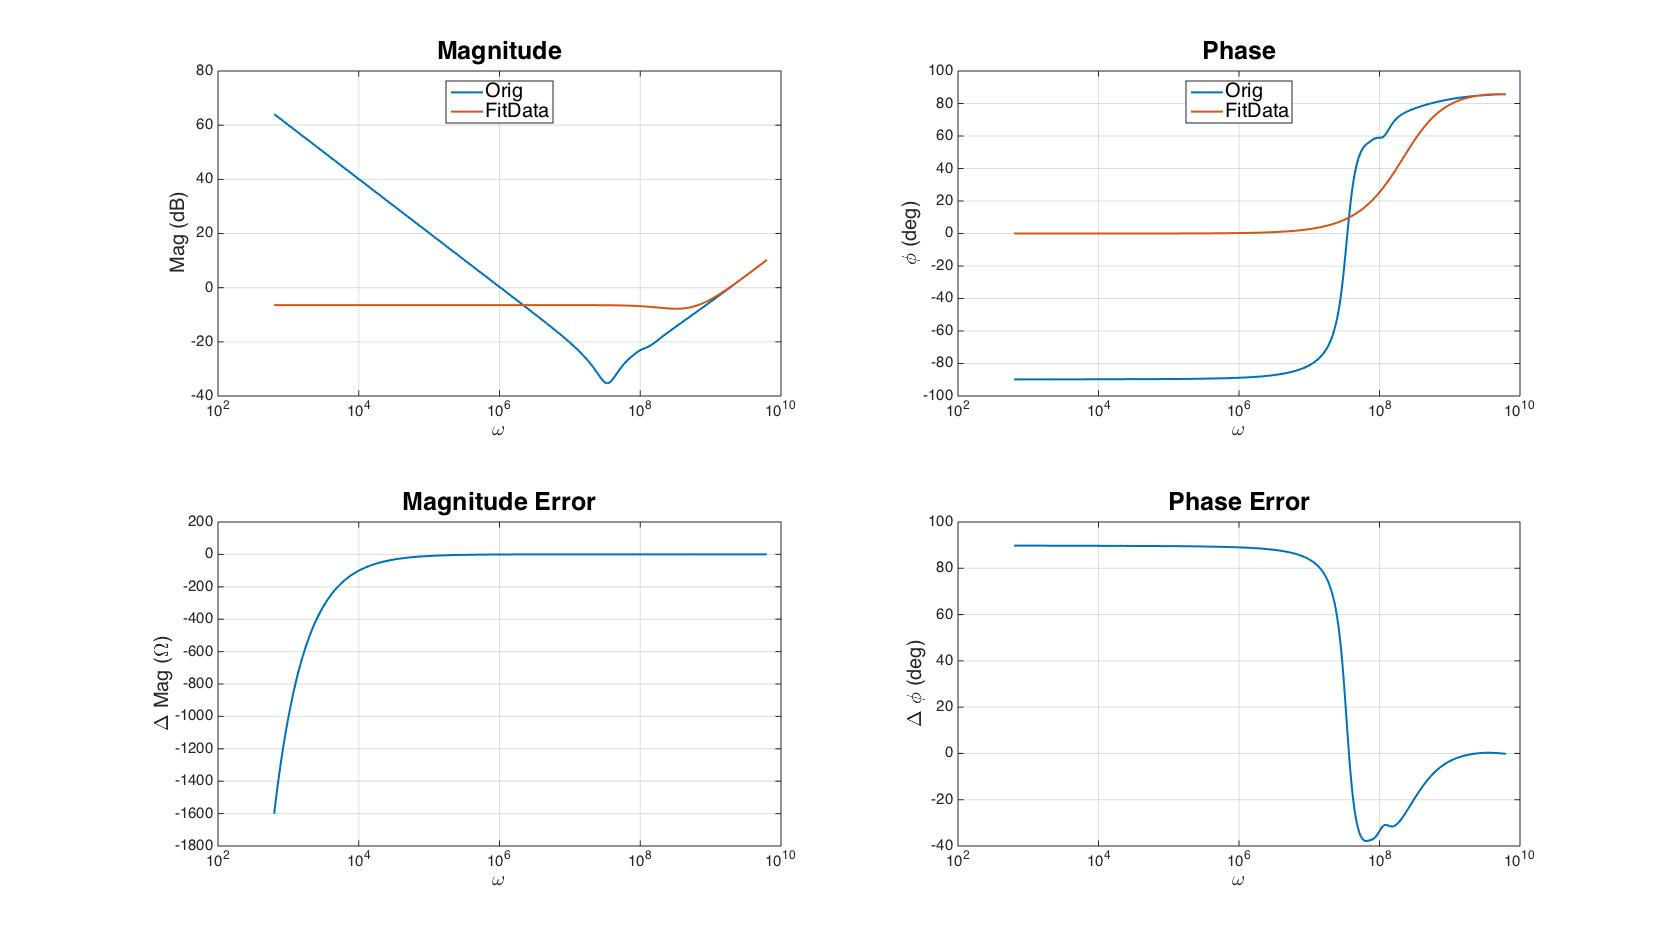
\includegraphics[keepaspectratio=true,width=6in]{./figures/regression/levy.jpg}
\centering
\caption{Levy's Technique}
\label{fig:levy}
\end{figure}



\subsubsection{Weighted LSE}
\label{sec:weightedLSE}
One improvement that can be made upon Levy's method is to iterate with a frequency dependent weighting function until the error term is minimized \cite{levy_iter}. By multiplying Levy's error function by the weighting term in Equation: \eqref{equ:iter_Weight}, we get Equation: \eqref{equ:iter_Err}, which can be used to obtain a new system of equations.
The $L$ subscript stands for the current iteration, while $L-1$ stands for the previous iteration.

\loadeq{iterWeight}
\loadeq{iterErr}

Equations \eqref{equ:Levy_Ans}, \eqref{equ:Levy_M}, \eqref{equ:Levy_N}, \& \eqref{equ:Levy_C} are the same, with Equations \eqref{equ:Levy_L}, \eqref{equ:Levy_S}, \eqref{equ:Levy_T}, \& \eqref{equ:Levy_U} being replaced with Equations: \eqref{equ:Iter_L}, \eqref{equ:Iter_S}, \eqref{equ:Iter_T}, \& \eqref{equ:Iter_U}.

\loadeq{IterL}
\loadeq{IterS}
\loadeq{IterT}
\loadeq{IterU}

Dependent upon the initial conditions and the model order, this particular method is not guaranteed to converge. Figure: \ref{fig:levyIter_Err1} was generated with an initial condition of $Q(jw_k) == 1$ and a model order of 7. It shows that, for this data set, the squared error of the magnitude and phase do not converge after a particular number of iterations. Furthermore, they do not reach their minimums at the same iteration. In order to select the desired iteration, the magnitude and phase squared plots are normalized as in Equation: \eqref{equ:ErrMin}. The index of the minimum of Figure: \ref{fig:levyIter_Err1} is selected as the best fit.

\loadeq{ErrMin}
\begin{figure}[ht!]
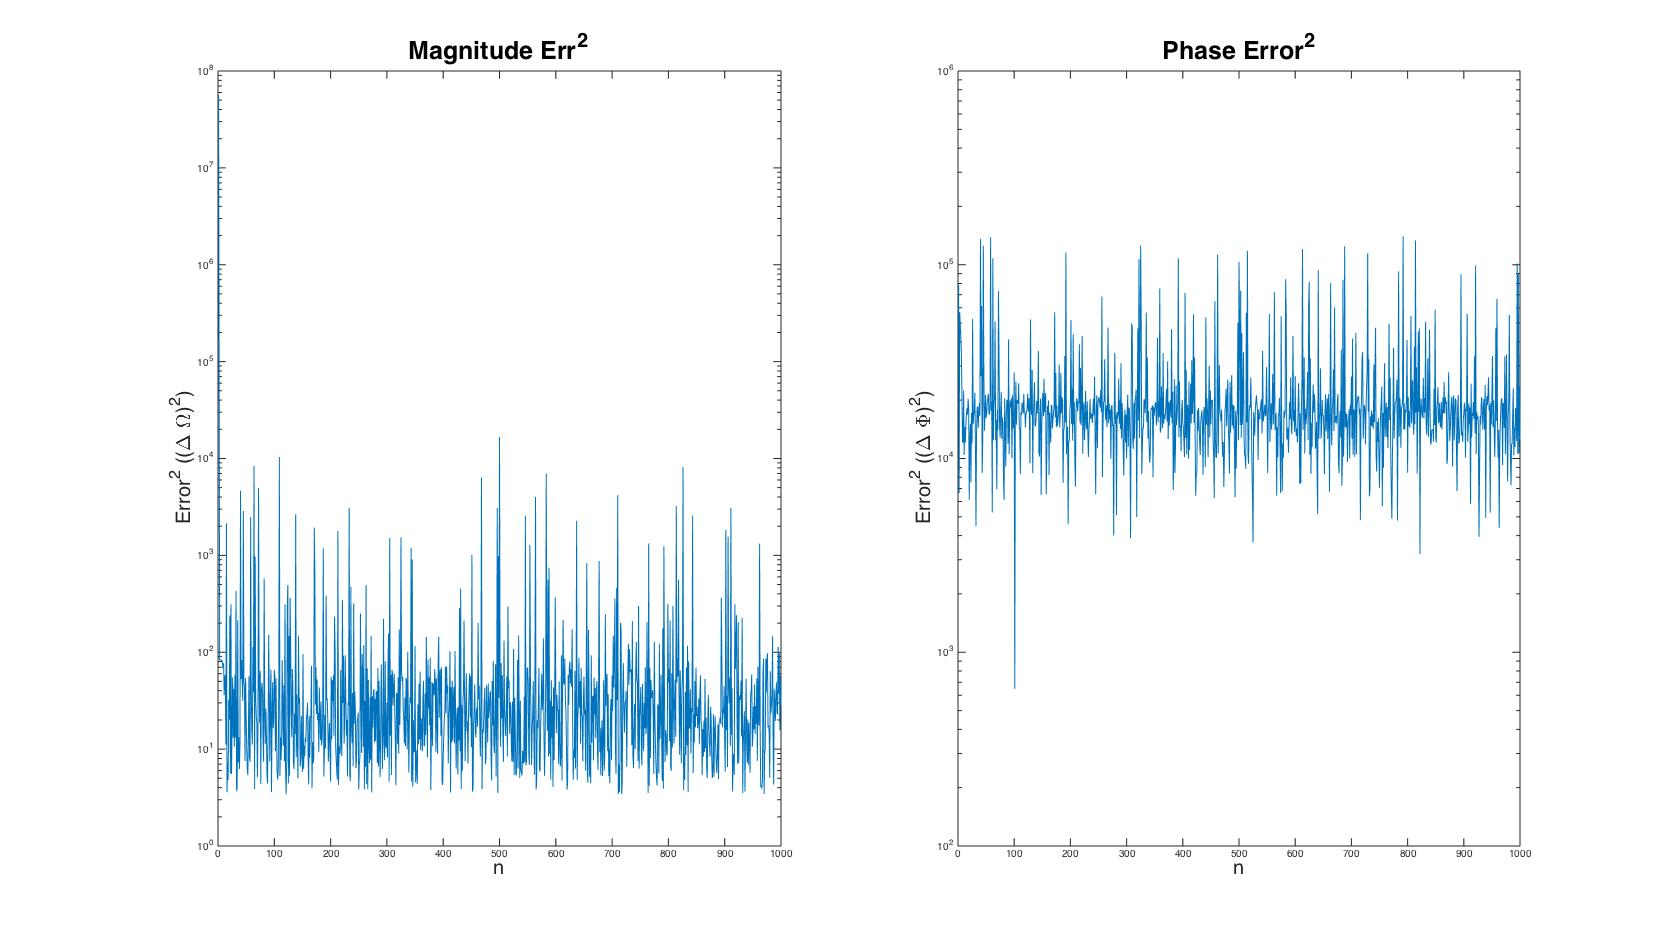
\includegraphics[keepaspectratio=true,width=6in]{./figures/modeling/levyIter_Err1.jpg}
\centering
\caption{LSE + Iteration -- Magnitude and Phase Error}
\label{fig:levyIter_Err1}
\end{figure}

% Run ./scripts/regression/run_levy_iter.m with numDeg = 7, denDeg = 7, and iterations = 100 to obtain this image.
\begin{figure}[ht!]
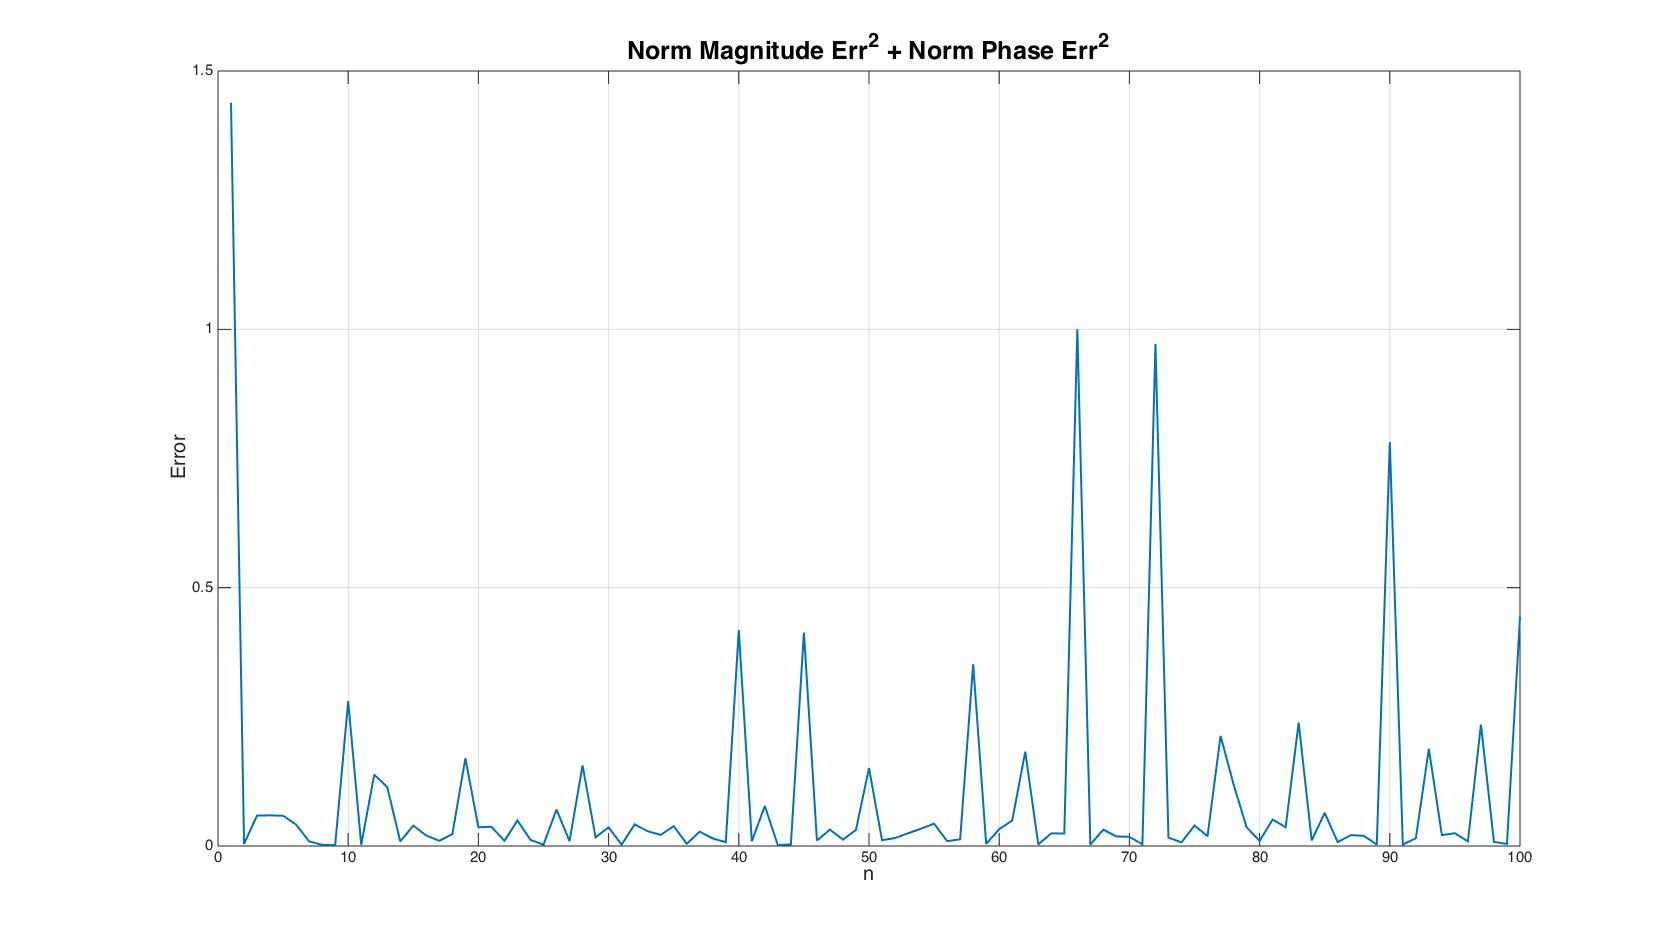
\includegraphics[keepaspectratio=true,width=6in]{./figures/regression/levyIter_Err2.jpg}
\centering
\caption{LSE + Iteration -- Combined Error}
\label{fig:levyIter_Err2}
\end{figure}



Figure: \ref{fig:levyIter} shows that this method can result in a much improved result over the Levy's original method, as seen in Figure: \ref{fig:levy}.

\begin{figure}
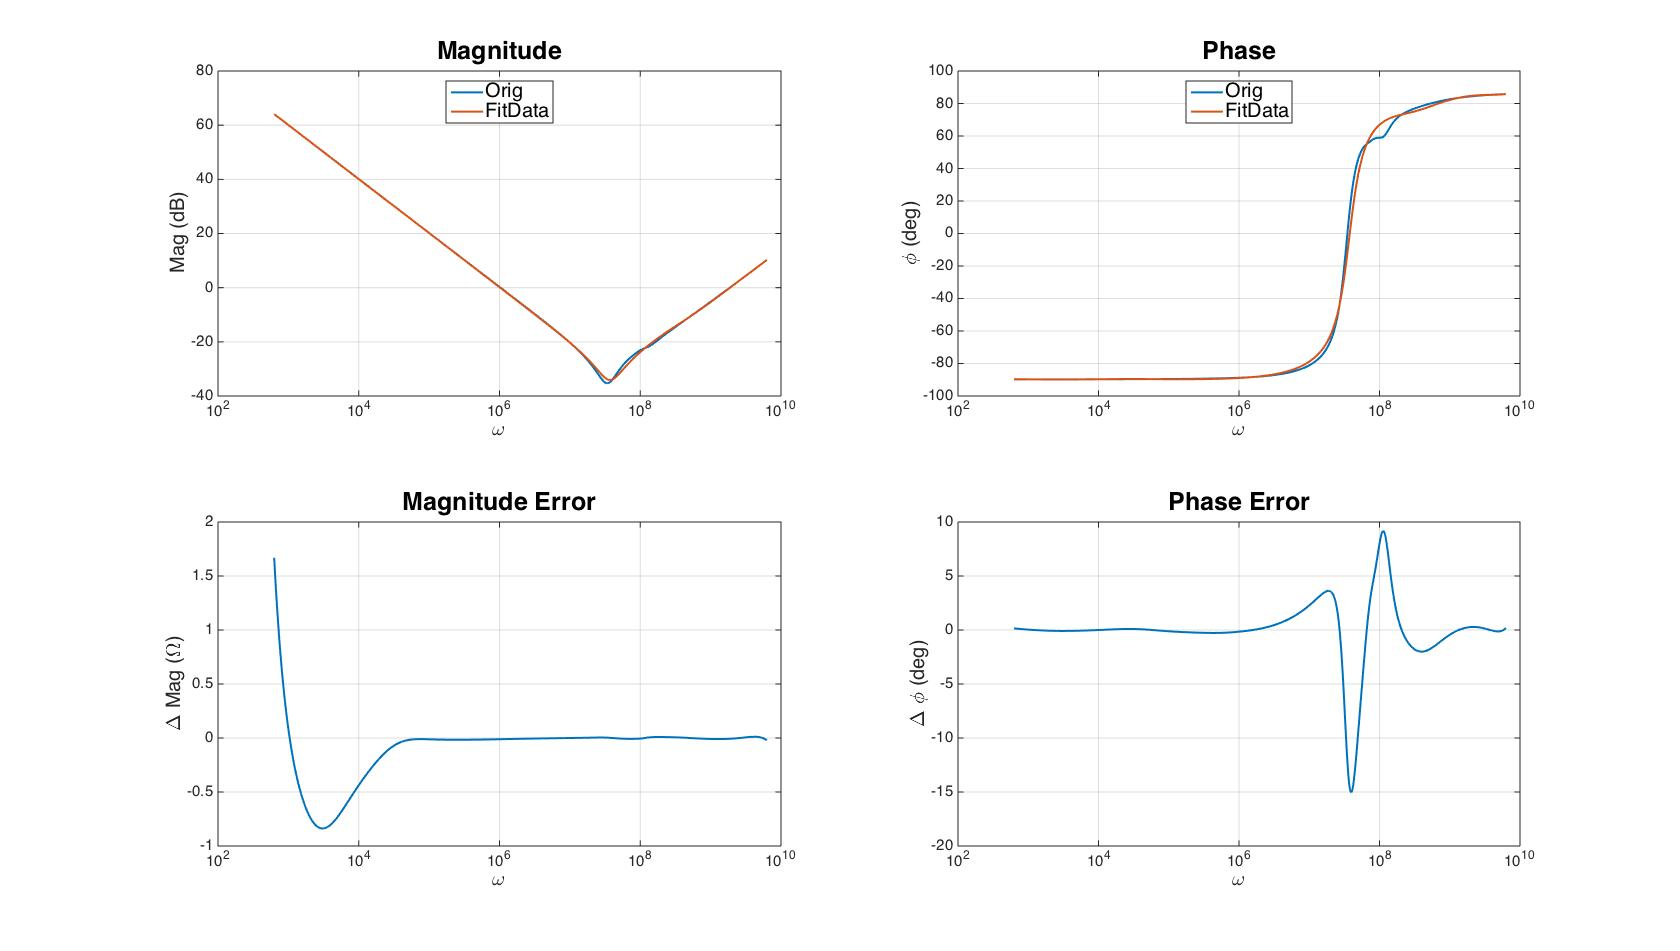
\includegraphics[keepaspectratio=true,width=6in]{./figures/modeling/levyIter.jpg}
\centering
\caption{LSE + Iteration}
\label{fig:levyIter}
\end{figure}


\subsection{Modeling}

This section will investigate a model which includes the most common parameters of merit. It will show how to fit the model to a data set with Levy's method described in Section: \ref{sec:RegressionAnalysis}, and will describe its effectiveness and limitations in doing so.
The data in Figure: \ref{fig:exCapData} used to fit against was generated from the model shown in Figure: \ref{fig:murataModel}. Since the model described in this section is of a smaller order than the model used to generate the data, there will be a loss of precision. This section will explore the error seen with the abbreviated model.

\subsubsection{Six Term Model}

The model shown in Figure: \ref{fig:fullModel} shows several of the most important parameters for a capacitor. It's impedance, shown in Equation: \eqref{equ:fullModelImpedance}, and generalized in Equation: \eqref{equ:fullModelPoly} can be used as the basis for a regression analysis.

\loadeq{fullModelImpedance}
\loadeq{fullModelPoly}

For this model, Equations: \eqref{equ:Levy_M}, \eqref{equ:Levy_N}, \& \eqref{equ:Levy_C} simplify down to Equations: \eqref{equ:fullModel_M}, \eqref{equ:fullModel_N}, \& \eqref{equ:fullModel_C}.

\loadeq{fullModelM}
\loadeq{FullModelN}

\begin{figure}[ht!]
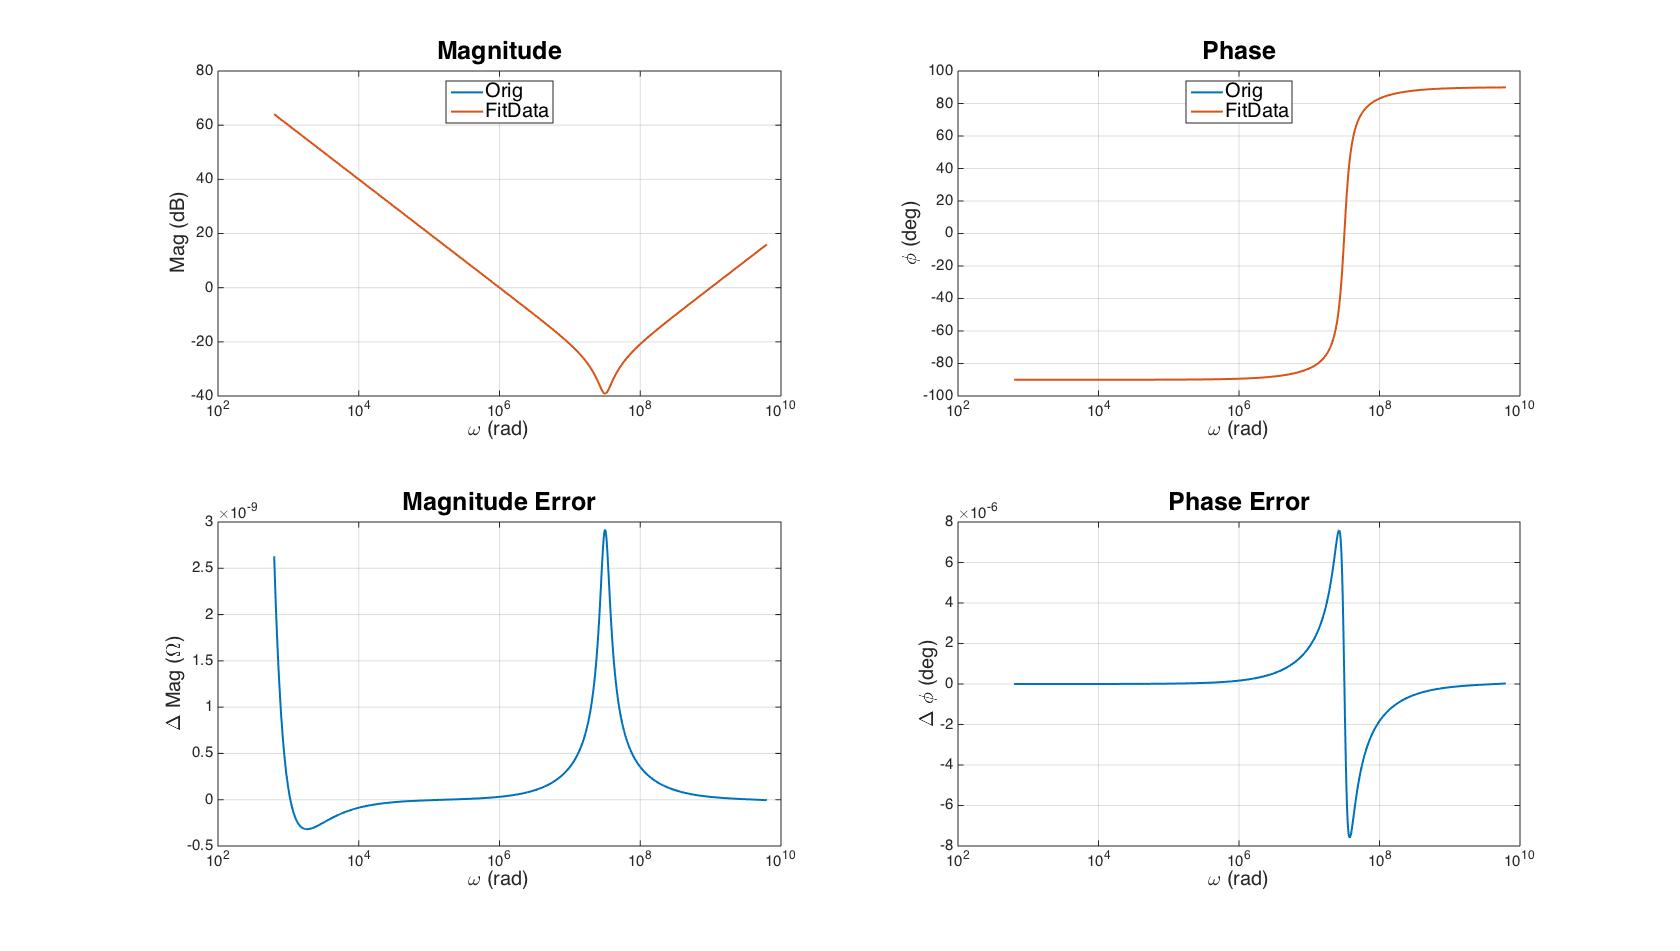
\includegraphics[keepaspectratio=true,width=6in]{./figures/regression/fullModel_test.jpg}
\centering
\caption{6 Term Model Validation}
\label{fig:fullModel_test}
\end{figure}

\begin{figure}[ht!]
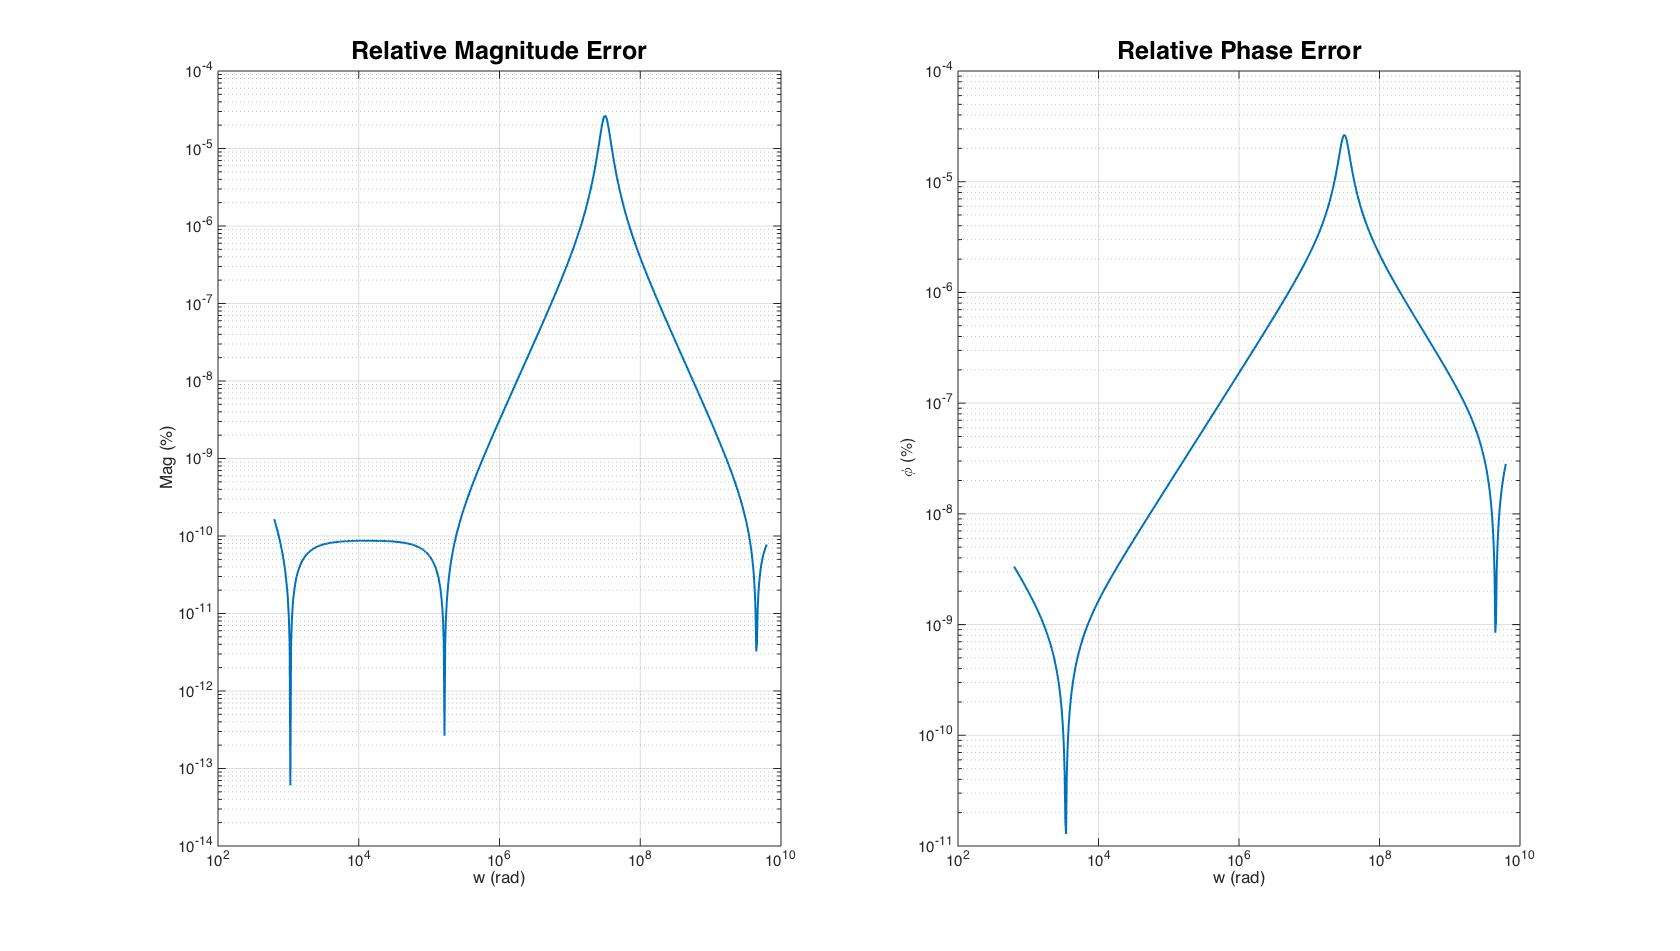
\includegraphics[keepaspectratio=true,width=6in]{./figures/regression/fullModel_testRel.jpg}
\centering
\caption{6 Term Model Validation: Relative Erorr}
\label{fig:fullModel_testRel}
\end{figure}

Figure: \ref{fig:fullModel_test} shows the results from simplifying the model in Figure: \ref{fig:murataModel} to the six term model and then applying this regression analysis to that model.
Figure: \ref{fig:fullModel_testRel} shows that the relative error in fitting this model to itself is negligible.

Using this model, the regression analysis method described in Section: \ref{sec:weightedLSE} generates the output seen in Figure: \ref{fig:fullModel_BadOutput}. The fit tracks the original data well, except at low frequencies and near resonance.

\begin{figure}[ht!]
\ifisPPT
\noindent\makebox[\textwidth]{\includegraphics[keepaspectratio=true,width=\paperwidth]{../figures/regression/fullModel_BadOutput.jpg}}
\else
\includegraphics[keepaspectratio=true,width=6in]{./figures/regression/fullModel_BadOutput.jpg}
\fi
\centering
\caption{6 Term Model: Bad Initilization}
\label{fig:fullModel_BadOutput}
\end{figure}


Substituting the polynomial coefficients seen in Equation: \eqref{equ:fullModel_BadOutputCoeff} into Equations: \eqref{equ:fullModel_CoeffEq_a0}-\eqref{equ:fullModel_CoeffEq_b2}, returns the model parameter values as seen in Equation: \eqref{equ:fullModel_BadOutputParams}.

\begin{align}
     a_0 &= R_E + R_L                                         \label{equ:fullModel_CoeffEq_a0} \\
     a_1 &= L_E + C_DR_DR_E + C_DR_DR_L + CR_ER_L + C_DR_ER_L \label{equ:fullModel_CoeffEq_a1} \\
     a_2 &= C_DL_ER_D + CL_ER_L + C_DL_ER_L + CC_DR_DR_ER_L   \label{equ:fullModel_CoeffEq_a2} \\
     a_3 &= CC_DL_ER_DR_L                                     \label{equ:fullModel_CoeffEq_a3} \\
     b_0 &= 1                                                 \label{equ:fullModel_CoeffEq_b0} \\
     b_1 &= C_DR_D + CR_L + C_DR_L                            \label{equ:fullModel_CoeffEq_b1} \\
     b_2 &= CC_DR_DR_L                                        \label{equ:fullModel_CoeffEq_b2}
\end{align}

Even though the polynomial coefficients gave an acceptable fit to the data, it resulted in unacceptable circuit parameters. Since $C$ and $R_D$ are negative, this model is not physically realizable.

\loadeq{FullModelBadOut}

This problem stems from the author's \cite{levy_iter} suggestion that the initial guess for $Q(jw_k) == 1$. While an initial guess is required to calculate the weighting function during the first iteration, this particular choice causes the problem seen in Equations: \eqref{equ:fullModel_BadInputCoeff} \& \eqref{equ:fullModel_BadInputParams} for this application. They show that this initial condition does not start with rational solution for the circuit parameters.

\loadeq{FullModelBadIn}

Starting instead with the rational set of circuit parameters seen in Equation: \eqref{equ:fullModel_GoodInputParams}, the starting coefficients are as seen in Equation: \eqref{equ:fullModel_GoodInputCoeff}.

\loadeq{FullModelGoodIn}

\begin{figure}[ht!]
\ifisPPT
\noindent\makebox[\textwidth]{\includegraphics[keepaspectratio=true,width=\paperwidth]{../figures/regression/fullModel_GoodOutput.jpg}}
\else
\includegraphics[keepaspectratio=true,width=6in]{./figures/regression/fullModel_GoodOutput.jpg}
\fi
\centering
\caption{6 Term Model: Good Initilization}
\label{fig:fullModel_GoodOutput}
\end{figure}


Figure: \ref{fig:fullModel_GoodOutput} shows a good fit across the frequency spectrum for both magnitude and phase. The model does deviate at resonance, but that is not surprising, as the number of parameters in the model is fairly low when compared with the model used to generate the data. As can be seen in Figure: \ref{fig:fullModel_Rel}, the relative error is the worst around resonance. It is at that point where there is simultaneously the lowest impedance and the sharpest feature in the plot.

The 6 term model described in this section provides a reasonable starting point for the capacitor characterization. As mentioned in the \nameref{sec:conclusion} and \nameref{sec:futureWork} sections, this model has enough accuracy to characterize new capacitors. Empirical testing is needed in order to determine if the model needs to be adjusted to better characterize a specific \gls{dut} of interest.

\begin{figure}[ht!]
\ifisPPT
\noindent\makebox[\textwidth]{\includegraphics[keepaspectratio=true,width=\paperwidth]{../figures/regression/fullModel_Rel.jpg}}
\else
\includegraphics[keepaspectratio=true,width=6in]{./figures/regression/fullModel_Rel.jpg}
\fi
\centering
\caption{6 Term Model: Relative Error}
\label{fig:fullModel_Rel}
\end{figure}


\subsection{Modeling Discharge Waveforms}
\label{sec:regDis}
Electric vehicles often rely on their DC-Link capacitors for acceleration. The capacitor's behavior in theses circumstances can be predicted by fittings its discharge curves to a model. Miller's model, seen in Figure: \ref{fig:superCap}, can be fit to a discharge waveform to show how an electrochemical capacitor delivers power. This task can be accomplished by using MATLAB's ``optimset'' and ``lsqnonlin'' functions in the method developed by Hokanson \cite{expFit}. The discharge current equation corresponding to Figure: \ref{fig:superCap} is omitted for brevity, but it can be generated by running the Mathematica code shown in the \nameref{app:disChargeEqs} Appendix.

